% F05: Pearson correlation heatmap (6x6) — hardcoded cells
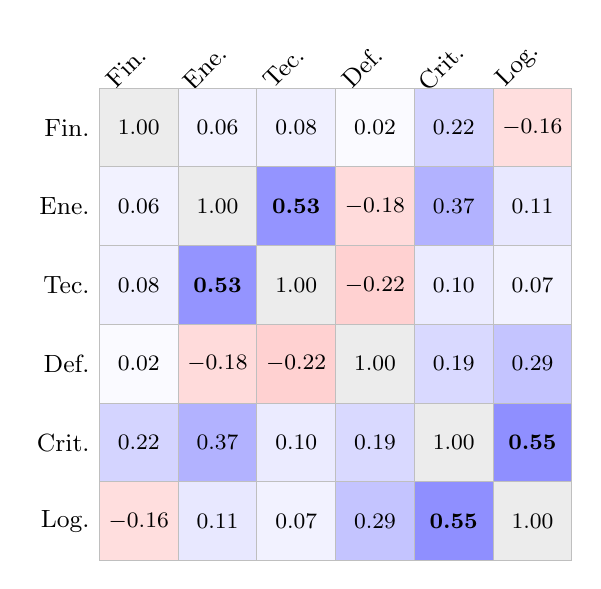
\begin{tikzpicture}
% Axis labels
\def\labels{{"Fin.","Ene.","Tec.","Def.","Crit.","Log."}}
% Row/column labels
\foreach \i in {0,...,5} {
  \pgfmathsetmacro{\lab}{\labels[\i]}
  \node[anchor=east, font=\small] at (0,-\i-0.5) {\lab};
  \node[anchor=south, font=\small, rotate=45] at (\i+0.5,0.1) {\lab};
}
% --- Row 0: Financial ---
\fill[gray!15]   (0, 0) rectangle ++(1,-1); \node[font=\footnotesize] at (0.5,-0.5) {1.00};
\fill[blue!5]    (1, 0) rectangle ++(1,-1); \node[font=\footnotesize] at (1.5,-0.5) {0.06};
\fill[blue!6]    (2, 0) rectangle ++(1,-1); \node[font=\footnotesize] at (2.5,-0.5) {0.08};
\fill[blue!2]    (3, 0) rectangle ++(1,-1); \node[font=\footnotesize] at (3.5,-0.5) {0.02};
\fill[blue!17]   (4, 0) rectangle ++(1,-1); \node[font=\footnotesize] at (4.5,-0.5) {0.22};
\fill[red!13]    (5, 0) rectangle ++(1,-1); \node[font=\footnotesize] at (5.5,-0.5) {$-$0.16};
% --- Row 1: Energy ---
\fill[blue!5]    (0,-1) rectangle ++(1,-1); \node[font=\footnotesize] at (0.5,-1.5) {0.06};
\fill[gray!15]   (1,-1) rectangle ++(1,-1); \node[font=\footnotesize] at (1.5,-1.5) {1.00};
\fill[blue!42]   (2,-1) rectangle ++(1,-1); \node[font=\footnotesize\bfseries] at (2.5,-1.5) {0.53};
\fill[red!14]    (3,-1) rectangle ++(1,-1); \node[font=\footnotesize] at (3.5,-1.5) {$-$0.18};
\fill[blue!30]   (4,-1) rectangle ++(1,-1); \node[font=\footnotesize] at (4.5,-1.5) {0.37};
\fill[blue!9]    (5,-1) rectangle ++(1,-1); \node[font=\footnotesize] at (5.5,-1.5) {0.11};
% --- Row 2: Technology ---
\fill[blue!6]    (0,-2) rectangle ++(1,-1); \node[font=\footnotesize] at (0.5,-2.5) {0.08};
\fill[blue!42]   (1,-2) rectangle ++(1,-1); \node[font=\footnotesize\bfseries] at (1.5,-2.5) {0.53};
\fill[gray!15]   (2,-2) rectangle ++(1,-1); \node[font=\footnotesize] at (2.5,-2.5) {1.00};
\fill[red!18]    (3,-2) rectangle ++(1,-1); \node[font=\footnotesize] at (3.5,-2.5) {$-$0.22};
\fill[blue!8]    (4,-2) rectangle ++(1,-1); \node[font=\footnotesize] at (4.5,-2.5) {0.10};
\fill[blue!5]    (5,-2) rectangle ++(1,-1); \node[font=\footnotesize] at (5.5,-2.5) {0.07};
% --- Row 3: Defence ---
\fill[blue!2]    (0,-3) rectangle ++(1,-1); \node[font=\footnotesize] at (0.5,-3.5) {0.02};
\fill[red!14]    (1,-3) rectangle ++(1,-1); \node[font=\footnotesize] at (1.5,-3.5) {$-$0.18};
\fill[red!18]    (2,-3) rectangle ++(1,-1); \node[font=\footnotesize] at (2.5,-3.5) {$-$0.22};
\fill[gray!15]   (3,-3) rectangle ++(1,-1); \node[font=\footnotesize] at (3.5,-3.5) {1.00};
\fill[blue!15]   (4,-3) rectangle ++(1,-1); \node[font=\footnotesize] at (4.5,-3.5) {0.19};
\fill[blue!23]   (5,-3) rectangle ++(1,-1); \node[font=\footnotesize] at (5.5,-3.5) {0.29};
% --- Row 4: Critical Inputs ---
\fill[blue!17]   (0,-4) rectangle ++(1,-1); \node[font=\footnotesize] at (0.5,-4.5) {0.22};
\fill[blue!30]   (1,-4) rectangle ++(1,-1); \node[font=\footnotesize] at (1.5,-4.5) {0.37};
\fill[blue!8]    (2,-4) rectangle ++(1,-1); \node[font=\footnotesize] at (2.5,-4.5) {0.10};
\fill[blue!15]   (3,-4) rectangle ++(1,-1); \node[font=\footnotesize] at (3.5,-4.5) {0.19};
\fill[gray!15]   (4,-4) rectangle ++(1,-1); \node[font=\footnotesize] at (4.5,-4.5) {1.00};
\fill[blue!44]   (5,-4) rectangle ++(1,-1); \node[font=\footnotesize\bfseries] at (5.5,-4.5) {0.55};
% --- Row 5: Logistics ---
\fill[red!13]    (0,-5) rectangle ++(1,-1); \node[font=\footnotesize] at (0.5,-5.5) {$-$0.16};
\fill[blue!9]    (1,-5) rectangle ++(1,-1); \node[font=\footnotesize] at (1.5,-5.5) {0.11};
\fill[blue!5]    (2,-5) rectangle ++(1,-1); \node[font=\footnotesize] at (2.5,-5.5) {0.07};
\fill[blue!23]   (3,-5) rectangle ++(1,-1); \node[font=\footnotesize] at (3.5,-5.5) {0.29};
\fill[blue!44]   (4,-5) rectangle ++(1,-1); \node[font=\footnotesize\bfseries] at (4.5,-5.5) {0.55};
\fill[gray!15]   (5,-5) rectangle ++(1,-1); \node[font=\footnotesize] at (5.5,-5.5) {1.00};
% Grid lines
\foreach \i in {0,...,5} {
  \foreach \j in {0,...,5} {
    \draw[gray!50, thin] (\j,-\i) rectangle ++(1,-1);
  }
}
\end{tikzpicture}
